\documentclass[11pt,a4paper]{report}

\usepackage{graphicx}
\usepackage{a4}
\usepackage{german}
\usepackage{acronym}
\usepackage{cite}


\newcommand{\thema}{$[$Thema der Bachelorarbeit$]$}
\newcommand{\schlagworte}{$[$Platz, f\"ur, spezifische, Schlagworte, zur, Ausarbeitung $]$}
\newcommand{\zusammenfassung}{$[$Text der Zusammenfassung etwa 150 Worte. Es soll der
	L"osungsweg beschrieben sein.$]$}
\newcommand{\ausgabedatum}{$[$Datum$]$}
\newcommand{\abgabedatum}{15.01.2016}
\newcommand{\autor}{Sandro Tonon}
\newcommand{\autorStrasse}{$[$Stra"se$]$}
\newcommand{\autorPLZ}{$[$PLZ$]$}
\newcommand{\autorOrt}{$[$Ort$]$}
\newcommand{\autorGeburtsort}{Test}
\newcommand{\autorGeburtsdatum}{02.07.1990}
\newcommand{\prueferA}{$[$Titel, Vor- und Zuname des 1. Pr"ufers$]$}
\newcommand{\prueferB}{$[$Titel, Vor- und Zuname des 2. Pr"ufers$]$}
\newcommand{\firma}{$[$HTWG oder Firmenname$]$}
\newcommand{\studiengang}{$[$Software-Engineering/Technische Informatik/Wirtschaftsinformatik$]$}


\begin{document}


\begin{titlepage}

\vspace*{-3.5cm}

\begin{flushleft}
\hspace*{-1cm} 
\includegraphics[width=15.7cm]{htwg-logo}
\end{flushleft}

\vspace{2.5cm}

\begin{center}
	\huge{
		\textbf{\thema} \\[5cm]
	}
	\Large{
		\textbf{\autor}} \\[6.5cm]
	\large{
		\textbf{Konstanz, \abgabedatum} \\[2.3cm]
	}
	
	\Huge{
		\textbf{{\sf BACHELORARBEIT}}
	}
\end{center}

\end{titlepage}

\thispagestyle{empty}
{
\setlength{\parskip}{0.5cm}
        \begin{center}
        \textbf{\huge BACHELORARBEIT}

        \textbf{zur Erlangung des akademischen Grades}

        \textbf{\Large Bachelor of Science (B. Sc.)}

        \textbf{an der}

        \textsf{\huge Hochschule Konstanz}\\
        {\small Technik, Wirtschaft und Gestaltung}

        \textsf{\Large Fakult"at Informatik} \\
        Studiengang \studiengang
        \end{center}
}
\begin{center}

\vspace*{2cm}

\begin{tabular}{p{3cm}p{10cm}}
Thema: & \multicolumn{1}{l}{\textbf{\large \thema}} \\[15ex]
Bachelorkandidat: & \autor, \autorStrasse, \autorPLZ{}  \autorOrt{} \\[15ex]
1. Pr"ufer: & \prueferA \\
2. Pr"ufer: & \prueferB \\[25ex]
Ausgabedatum: & \ausgabedatum \\
Abgabedatum: & \abgabedatum \\
\end{tabular}
\end{center}

\begin{center}
{\Large \textbf{Zusammenfassung (Abstract)}}
\end{center}

\bigskip

\begin{center}
	\begin{tabular}{p{2.8cm}p{10cm}}
		Thema: & \thema \\
		 & \\
		Bachelorkandidat: & \autor \\
		 & \\
		Firma: & \firma \\
		 & \\
		Betreuer: & \prueferA  \\[.5ex]
		 &  \prueferB \\
		 & \\
		Abgabedatum: & \abgabedatum \\
		 & \\
		Schlagworte: & \schlagworte \\
		 & \\
	\end{tabular}
\end{center}

\bigskip

\noindent
\zusammenfassung
\chapter*{Ehrenw"ortliche Erkl"arung}
\addcontentsline{toc}{chapter}{Ehrenw"ortliche Erkl"arung}

Hiermit erkl"are ich
\textit{\autor, geboren am \autorGeburtsdatum{} in \autorGeburtsort{}}, dass ich\\

\begin{tabular}{lp{12cm}}
(1) & meine Bachelorarbeit mit dem Titel \\[1em]
& \textbf{\thema} \\[1em]
& selbstst"andig und ohne fremde Hilfe angefertigt und keine anderen als die angef"uhrten Hilfen benutzt habe;\\[1em]
(2) & die "Ubernahme w"ortlicher Zitate, von Tabellen, Zeichnungen, Bildern und
Programmen aus der Literatur oder anderen Quellen (Internet) sowie die Verwendung
der Gedanken anderer Autoren an den entsprechenden Stellen innerhalb der Arbeit
gekennzeichnet habe.\\
\end{tabular}

\vspace*{1cm}

\noindent
Ich bin mir bewusst, dass eine falsche Erkl"arung rechtliche Folgen haben wird.\\

\vspace*{3cm}

\noindent
Konstanz, \abgabedatum \hfill \begin{tabular}{c} \\ \\ \rule{5cm}{1pt} \\ (Unterschrift)\end{tabular}


% Inhaltsverzeichnis anzeigen
\tableofcontents

\newpage


\section{Custom Elements}\label{custom-elements}

Der erste Begriff unter dem Dachbegriff Web Components sind die Custom
Elements, die es ermöglichen eigene HTML Elemente zu definieren.

\subsection{Einleitung}\label{einleitung}

Webseiten werden mit sogenannten Elementen, oder auch Tags, aufgebaut.
Das Set an verfügbaren Elementen wird vom W3C definiert und
standardisiert. Somit ist die Auswahl an den verfügbaren Elementen stark
begrenzt und nicht von Entwicklern erweiterbar, sodass diese ihre
eigenen, von ihrer Applikation benötigten Elemente, definieren können.
Betrachtet man den Quelltext einer Webseite im Internet, wird schnell
deutlich, worin das Problem liegt.

\begin{figure}[htbp]
\centering
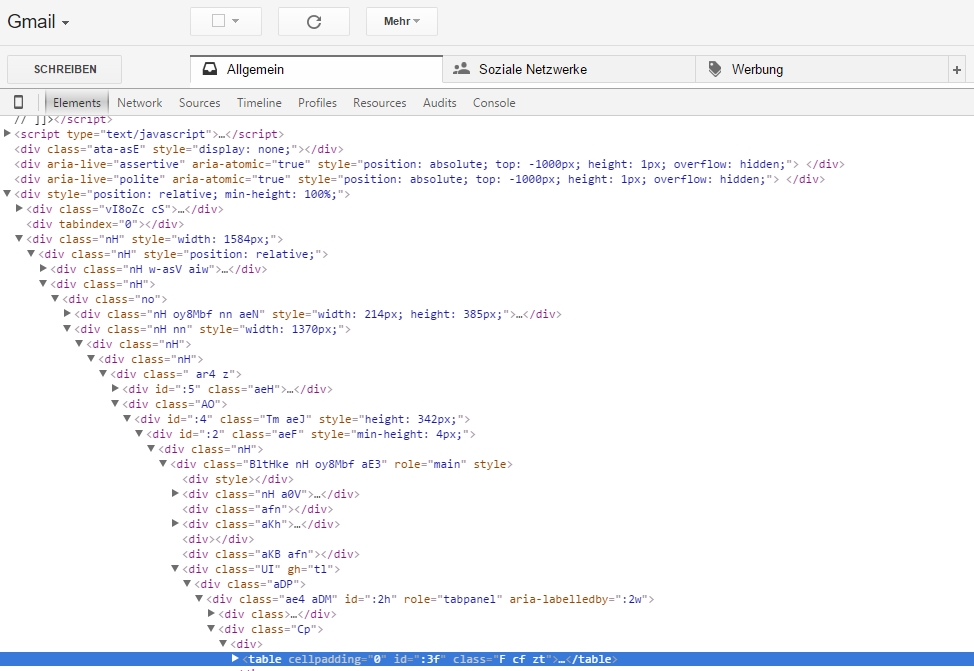
\includegraphics{images/1-custom-elements-div-suppe.jpg}
\caption{Bild: Webseite mit semantisch nicht aussagekräftigem Markup}
\end{figure}

Die Webseite der Google Mail Applikation ist stark geschachtelt in
\texttt{\textless{}div\textgreater{}}-Elemente. Diese sind notwendig um
der Webseite die gewünschte Funktionalität und Aussehen zu verleihen.
Die Probleme dieser Struktur bzw. des DOM sind deutlich: Es ist sehr
schwer zu erkennen, welches Element nun was darstellt und welche
Funktion hat. Abgesehen von der fehlenden, schnell ersichtlichen
Semantik, also der Zuordnung der Bedeutung zu einem Element, ist der
gesamte DOM nur schwer wartbar. Dieser Problematik widmen sich die
Custom Elements. Sie bieten eine neue API, welche es ermöglicht eigene,
semantisch aussagekräftige, HTML-Elemente sowie deren Eigenschaften und
Funktionen zu definieren. Würde das obige Beispiel nun also mit Hilfe
von Custom Elements umgesetzt werden, so könnte der zugehörige DOM
folgender Maßen aussehen {[}citeulike:13844982{]}.

\begin{Shaded}
\begin{Highlighting}[]
\KeywordTok{<hangout-module>}
  \KeywordTok{<hangout-chat}\OtherTok{ from=}\StringTok{"Paul, Addy"}\KeywordTok{>}
    \KeywordTok{<hangout-discussion>}
      \KeywordTok{<hangout-message}\OtherTok{ from=}\StringTok{"Paul"}\OtherTok{ profile=}\StringTok{"profile.png"}
\OtherTok{          profile=}\StringTok{"118075919496626375791"}\OtherTok{ datetime=}\StringTok{"2013-07-17T12:02"}\KeywordTok{>}
        \KeywordTok{<p>}\NormalTok{Feelin' this Web Components thing.}\KeywordTok{</p>}
        \KeywordTok{<p>}\NormalTok{Heard of it?}\KeywordTok{</p>}
      \KeywordTok{</hangout-message>}
    \KeywordTok{</hangout-discussion>}
  \KeywordTok{</hangout-chat>}
  \KeywordTok{<hangout-chat>}\NormalTok{...}\KeywordTok{</hangout-chat>}
\KeywordTok{</hangout-module>}
\end{Highlighting}
\end{Shaded}

Die Spezifikation des W3C ermöglicht nicht nur das Erstellen eigener
Elemente, sondern auch das Erstellen von eigenen Elementen, die native
Elemente erweitern. Somit können die APIs von nativen HTML Elementen um
eigene Eigenschaften und Funktionen erweitert werden. Dies ermöglicht
es, eigene gewünschte Funktionalitäten in eigens erstellten HTML
Elementen zu bündeln.

\subsection{Neue Elemente
registrieren}\label{neue-elemente-registrieren}

Um nun ein eigenes Custom Element zu definieren, muss der Name des
Custom Elements, laut der W3C Spezifikation, zwingend einen Bindestrich
enthalten, beispielsweise \texttt{my-element}. Somit ist gewährleistet,
dass der Parser des Browsers die Custom Elements von den nativen
Elementen unterscheiden kann {[}citeulike:13845061{]}. Ein neues Element
wird mittels JavaScript mit der Funktion
\texttt{var\ MyElement\ =\ document.registerElement(\textquotesingle{}my-element\textquotesingle{});}
registriert. Zusätzlich zum Namen des Elementes, kann optional der
Prototyp des Elementes angegeben werden. Dieser ist jedoch standardmäßig
ein \texttt{HTMLElement}, somit also erst wichtig, wenn es darum geht
vorhandene Elemente zu erweitern, auf dieses Thema wird jedoch gesondert
eingegangen. Durch das Registrieren des Elementes wird es in die
Registry des Browsers geschrieben, welche dazu verwendet wird die
Definitionen der HTML-Elemente aufzulösen. Nachdem das Element
registriert wurde, muss es zunächst mittels
\texttt{document.createElement(tagName)} erzeugt werden, der
\texttt{tagName} ist hierbei der Name des zuvor registrierten Elementes.
Danach kann es per JavaScript oder HTML-Deklaration im Dokument
verwendet werden {[}citeulike:13844979{]}.

JavaScript

\begin{Shaded}
\begin{Highlighting}[]
\KeywordTok{var} \NormalTok{myelement }\OperatorTok{=} \VariableTok{document}\NormalTok{.}\AttributeTok{createElement}\NormalTok{(}\StringTok{'my-element'}\NormalTok{)}\OperatorTok{;}
\VariableTok{document}\NormalTok{.}\VariableTok{body}\NormalTok{.}\AttributeTok{appendChild}\NormalTok{(myelement)}\OperatorTok{;}
\end{Highlighting}
\end{Shaded}

HTML

\begin{Shaded}
\begin{Highlighting}[]
\KeywordTok{<div}\OtherTok{ class=}\StringTok{"some-html"}\KeywordTok{>}
  \KeywordTok{<my-element><my-element>}
\KeywordTok{</div>}
\end{Highlighting}
\end{Shaded}

\subsection{Vorteile von Custom
Elements}\label{vorteile-von-custom-elements}

Ist ein Element noch nicht definiert und nicht beim Browser registiert,
steht aber im Markup der Webseite, beispielsweise
\texttt{\textless{}myelement\textgreater{}}, wird dies kein Fehler
verursachen, da dieses Element das Interface von
\texttt{HTMLUnkownElement} benutzen muss {[}citeulike:13851253{]}. Ist
es jedoch definiert oder beim Browser registriert worden, beispielsweise
\texttt{\textless{}my-element\textgreater{}}, so benutzt es das
Interface eines \texttt{HTMLElement}. Dies bedeutet, dass für neue
eigene Elemente, eigene APIs für dieses Element erzeugt werden können,
indem eigene Eigenschaften und Methoden hinzugefügt werden
{[}citeulike:13844982{]}. Eigene Elemente, mit einem spezifischen
Eigenverhalten und Aussehen, wie beispielsweise ein neuer Video-Player,
sind dadurch mit einem Tag, statt mit einem Gerüst aus Divs oder
ähnlichen umsetzbar.

\subsubsection{Nachteil}\label{nachteil}

Ein Custom Element, das zwar standardkonform deklariert oder erstellt,
aber noch nicht beim Browser registriert wurde, ist es ein
\texttt{Unresolved\ Element}. Steht dieses Element am Anfang des DOM,
wird jedoch erst später registriert, kann es nicht von CSS angesprochen
werden. Dadurch kann ein FOUC entstehen, was bedeutet, dass das Element
beim Laden der Seite nicht gestylt dargestellt wird, sondern erst
nachdem es registriert wurde, das definierte Aussehen übernimmt. Um dies
zu verhindern, sieht die HTML Spezifikation eine neue CSS-Pseudoklasse
\texttt{:unresolved} vor, welche deklarierte aber nicht registrierte
Elemente anspricht. Somit können diese Elemente initial beim Laden der
Seite ausgeblendet, und nach dem Registrieren wieder eingeblendet
werden. Dadurch wird ein ungewolltes Anzeigen von ungestylten Inhalten
verhindert {[}citeulike:13844984{]}.

\begin{verbatim}
my-element:unresolved {
  display: none;
}
\end{verbatim}

\subsection{Vorhandene Elemente erweitern (Type
extensions)}\label{vorhandene-elemente-erweitern-type-extensions}

Statt neue Elemente zu erzeugen können sowohl native HTML Elemente, als
auch eigene erstellte HTML Elemente, um Funktionen und Eigenschaften
erweitert werden, auch ``Type extensions'' genannt. Diese erben von
einem spezifischen HTMLElement, also ``Element X ist ein Y''. Zusätzlich
zum Namen des erweiterten Elementes wird nun der Prototyp, sowie der
Name des zu erweiternden Elementes der \texttt{registerElement}-Funktion
als Parameter übergeben. Soll nun ein erweitertes
\texttt{button}-Element erzeugt werden, muss folgendes gemacht werden:

\begin{Shaded}
\begin{Highlighting}[]
\KeywordTok{var} \NormalTok{ButtonExtendedProto }\OperatorTok{=} \VariableTok{document}\NormalTok{.}\AttributeTok{registerElement}\NormalTok{(}\StringTok{'button-extended'}\OperatorTok{,} \OperatorTok{\{}
  \DataTypeTok{prototype}\OperatorTok{:} \VariableTok{Object}\NormalTok{.}\AttributeTok{create}\NormalTok{(}\VariableTok{HTMLButtonElement}\NormalTok{.}\AttributeTok{prototype}\NormalTok{)}\OperatorTok{,}
  \DataTypeTok{extends}\OperatorTok{:} \StringTok{'button'}
\OperatorTok{\}}\NormalTok{)}\OperatorTok{;}
\end{Highlighting}
\end{Shaded}

Das registrierte, erweiterte Element kann nun mit dem Namen des zu
erweiternden Elementes als erstem Parameter und dem Namen des
erweiterten Elementes als zweitem Parameter erzeugt werden. Alternativ
kann es auch mit Hilfe des Konstruktors erzeugt werden
{[}citeulike:13752379{]}.

JavaScript:

\begin{Shaded}
\begin{Highlighting}[]
\KeywordTok{var} \NormalTok{buttonExtended  }\OperatorTok{=} \VariableTok{document}\NormalTok{.}\AttributeTok{createElement}\NormalTok{(}\StringTok{'button'}\OperatorTok{,} \StringTok{'button-extended'}\NormalTok{)}\OperatorTok{;}

\CommentTok{// Alternativ}
\KeywordTok{var} \NormalTok{buttonExtended }\OperatorTok{=} \KeywordTok{new} \AttributeTok{ButtonExtendedProto}\NormalTok{()}\OperatorTok{;}
\end{Highlighting}
\end{Shaded}

Um es nun im DOM zu benutzen, muss der Name des erweiterten Elementes
via dem Attribut \texttt{is="elementName"} des erweiternden Elementes
angegeben werden.

HTML:

\begin{Shaded}
\begin{Highlighting}[]
  \KeywordTok{<div}\OtherTok{ class=}\StringTok{"wrapper"}\KeywordTok{>}
    \KeywordTok{<button}\OtherTok{ is=}\StringTok{"button-extended"}\KeywordTok{></button>}
  \KeywordTok{</div>}
\end{Highlighting}
\end{Shaded}

\subsubsection{Verwendung bei Github}\label{verwendung-bei-github}

Eine Umsetzung der Type extensions ist auf der Webseite von GitHub zu
finden. Dort werden die ``Latest commit'' Angaben eines Repositories als
ein erweitertes time-Element dargestellt. Statt des Commit-Datums und
der Zeit, wird die berechnete Zeit seit dem letzten Commit angezeigt.

\begin{figure}[htbp]
\centering
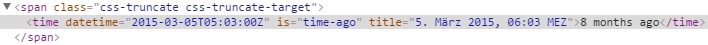
\includegraphics{images/1-custom-elements-github-time-element.jpg}
\caption{Bild: Github Einsatz eines Custom Element}
\end{figure}

GitHub verwendet hierzu ein selbst erzeugtes \texttt{time-ago}-Element,
welches eine Type extension auf Basis des \texttt{time}-Elementes
umsetzt. Mittels dem \texttt{datetime}-Attribut wird die absolute Zeit
des Commits an das interne JavaScript weitergegeben. Als Inhalt des
\texttt{time}-Elements wird dann die mit JavaScript berechnete relative
Zeit ausgegeben. Falls der Browser nun keine Custom Elements unterstützt
oder JavaScript deaktiviert ist, wird dennoch das nicht erweiterte,
native HTML \texttt{time} Element mit der absoluten Zeit angezeigt.

\subsection{Eigenschaften und Methoden
definieren}\label{eigenschaften-und-methoden-definieren}

Anhand des Beispiels auf GitHub wird deutlich, wie ein Custom Element
eingesetzt werden kann, jedoch sind die internen JavaScript Mechanismen
nicht ersichtlich. Custom Elements machen allerdings erst so richtig
Sinn, wenn man für diese auch eigene Eigenschaften und Methoden
definieren kann. Wie bei nativen HTML Elementen, ist das auch bei Custom
Elements auf analoge Weise möglich {[}citeulike:13844979{]}. So kann
einem Element eine Funktion zugewiesen werden, in dem diese dessen
Prototyp mittels einem noch freien Namen angegeben wird. Selbiges gilt
für eine neue Eigenschaft.

\begin{Shaded}
\begin{Highlighting}[]
\CommentTok{// Methode definieren}
\VariableTok{ButtonExtendedProto}\NormalTok{.}\AttributeTok{alert} \OperatorTok{=} \KeywordTok{function} \NormalTok{() }\OperatorTok{\{}
  \AttributeTok{alert}\NormalTok{(}\StringTok{'foo'}\NormalTok{)}\OperatorTok{;}
\OperatorTok{\};}

\CommentTok{// Eigenschaft definieren}
\VariableTok{ButtonExtendedProto}\NormalTok{.}\AttributeTok{answer} \OperatorTok{=} \DecValTok{42}\OperatorTok{;}
\end{Highlighting}
\end{Shaded}

\subsection{Custom Element Life Cycle
Callbacks}\label{custom-element-life-cycle-callbacks}

Custom Elements bieten eine standardisierte API an speziellen Methoden,
den \texttt{Custom\ Element\ Life\ Cycle\ Callbacks}, welche es
ermöglichen Funktionen zu unterschiedlichen Zeitpunkten, vom
Registrieren bis zum löschen eines Custom Elements, auszuführen. Diese
ermöglichen es zu bestimmen, wann und wie ein bestimmter Code des Custom
Elements ausgeführt werden soll.

\paragraph{createdCallback}\label{createdcallback}

Die \texttt{createdCallback}-Funktion Wird ausgeführt, wenn eine Instanz
des Custom Elements erzeugt mittels
\texttt{var\ mybutton\ =\ document.createElement(\textquotesingle{}custom-element\textquotesingle{})}
wird.

\paragraph{attachedCallback}\label{attachedcallback}

Die \texttt{attachedCallback}-Funktion wird ausgeführt, wenn ein Custom
Element dem DOM mittels \texttt{document.body.appendChild(mybutton)}
angehängt wird.

\paragraph{detachedCallback}\label{detachedcallback}

Die \texttt{detachedCallback}-Funktion wird ausgeführt, wenn ein Custom
Element aus dem DOM mittels \texttt{document.body.removeChild(mybutton)}
entfernt wird.

\paragraph{attributeChangedCallback}\label{attributechangedcallback}

Die \texttt{attributeChangedCallback}-Funktion wird ausgeführt, wenn ein
Attribut eines Custom Elements mittels \texttt{MyElement.setAttribute()}
geändert wird.

So können die Life Cycle Callbacks für ein neues erweitertes
Button-Element wie folgt definiert werden {[}citeulike:13844988{]}.

\begin{Shaded}
\begin{Highlighting}[]
\KeywordTok{var} \NormalTok{ButtonExtendedProto }\OperatorTok{=} \VariableTok{Object}\NormalTok{.}\AttributeTok{create}\NormalTok{(}\VariableTok{HTMLElement}\NormalTok{.}\AttributeTok{prototype}\NormalTok{)}\OperatorTok{;}

\VariableTok{ButtonExtendedProto}\NormalTok{.}\AttributeTok{createdCallback} \OperatorTok{=} \KeywordTok{function}\NormalTok{() }\OperatorTok{\{}\NormalTok{...}\OperatorTok{\};}
\VariableTok{ButtonExtendedProto}\NormalTok{.}\AttributeTok{attachedCallback} \OperatorTok{=} \KeywordTok{function}\NormalTok{() }\OperatorTok{\{}\NormalTok{...}\OperatorTok{\};}

\KeywordTok{var} \NormalTok{ButtonExtended }\OperatorTok{=} \VariableTok{document}\NormalTok{.}\AttributeTok{registerElement}\NormalTok{(}\StringTok{'button-extended'}\OperatorTok{,} \OperatorTok{\{}\DataTypeTok{prototype}\OperatorTok{:} \NormalTok{ButtonExtendedProto}\OperatorTok{\}}\NormalTok{)}\OperatorTok{;}
\end{Highlighting}
\end{Shaded}

\subsection{Styling von Custom
Elements}\label{styling-von-custom-elements}

Das Styling von eigenen Custom Elements funktioniert analog dem Styling
von nativen HTML Elementen in dem der Name des Elementes als CSS
Selektor angegeben wird. Erweiterte Elemente können mittels dem
Attribut-Selektor in CSS angesprochen werden {[}citeulike:13844979{]}.

\begin{Shaded}
\begin{Highlighting}[]
\CommentTok{/* Eigenes Custom Element */}
\NormalTok{my-element }\KeywordTok{\{}
  \KeywordTok{color:} \DataTypeTok{black}\KeywordTok{;}
\KeywordTok{\}}

\CommentTok{/* Erweitertes natives HTML Element*/}
\CharTok{[is=}\StringTok{"button-extended"}\CharTok{]} \KeywordTok{\{}
  \KeywordTok{color:} \DataTypeTok{black}\KeywordTok{;}
\KeywordTok{\}}
\end{Highlighting}
\end{Shaded}

\subsection{Browserunterstützung}\label{browserunterstuxfctzung}

HTML Imports sind noch nicht vom W3C standardisiert, sondern befinden
sich noch im Status eines ``Working Draft'' {[}citeulike:13845061{]}.
Sie werden deshalb bisher nur von Google Chrome ab Version 43 und Opera
ab Version 33 nativ unterstützt.

\begin{figure}[htbp]
\centering
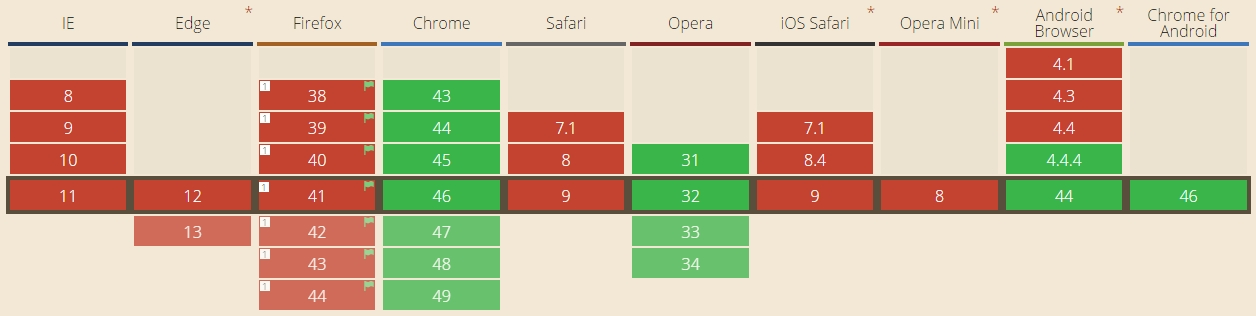
\includegraphics{images/1-custom-elements-browserunterstuetzung.jpg}
\caption{Bild: Browserunterstützung von Custom Elements}
\end{figure}

\subsection{Quellen}\label{quellen}

\begin{itemize}
\tightlist
\item
  {[}citeulike:13844979{]} Jarrod Overson \& Jason Strimpel, Developing
  Web Components, O'Reilly 2015, S.127-138
\item
  {[}citeulike:13845061{]} W3C Custom Elements,
  http://w3c.github.io/webcomponents/spec/custom/\#concepts
\item
  {[}citeulike:13752379{]} Eiji Kitamura, Introduction to Custom
  Elements,
  http://webcomponents.org/articles/introduction-to-custom-elements/
\item
  http://w3c.github.io/webcomponents/spec/custom/
\item
  {[}citeulike:13844982{]} Eric Bidelman, Custom Elements,
  http://www.html5rocks.com/en/tutorials/webcomponents/customelements/
\item
  {[}citeulike:13844983{]} Can I Use,
  http://caniuse.com/\#feat=custom-elements
\item
  {[}citeulike:13844984{]} Peter Gasstton, A Detailed Introduction To
  Custom Elements,
  http://www.smashingmagazine.com/2014/03/introduction-to-custom-elements/
\item
  {[}citeulike:13844988{]} Raoul Schaffranek, Web Components -- eine
  Einführung,
  https://blog.selfhtml.org/2014/12/09/web-components-eine-einfuehrung/
\item
  {[}citeulike:13851253{]} WHATWG, HTML Specification,
  https://html.spec.whatwg.org/multipage/dom.html\#htmlunknownelement
\end{itemize}




\section{Abkürzungsverzeichnis}
\begin{acronym}

 \acro{bzw.}{beziehungsweise}
 \acro{HTML}{Hypertext Markup Language}
 \acro{W3C}{World Wide Web Consortium}
 \acro{DOM}{Document Object Model}
 \acro{CSS}{Cascading Style Sheets}
 \acro{API}{Application Programming Interface}
 \acro{FOUC}{Flash Of Unstyled Content}
 \acro{LIFO}{Last In First Out}

\end{acronym}
\end{document}



\bibliographystyle{plain}
\bibliography{library}
\end{document}

